\documentclass{book}
\usepackage{commeunjeustyle}
\begin{document}
\chapter*{Probabilité discrète}
Lors du cours sur les probabilité finies, nous avons posé le cadre probabiliste afin de modéliser une expérience aléatoire dans les issues sont finies. Ce cours étend le cadre pour aussi modéliser une expérience aléatoire dont les issues sont \impo{dénombrables finies ou infinies}, c'est à dire que l'on peut effectuer une énumération finie ou infinie des issues de l'expérience aléatoire.  Nous énoncerons uniquement les extensions et les nouvelles notions.   
 

\section{Extension  de la modélisation probabilistes pour un univers dénombrable}
\subsection{Axiomes des probabilité. Premières propriétés}
\begin{Exemple}[Première fois pile]
Pour le lancer d'une pièce jusqu'à la première obtention de pile. L'univers est dénombrable $\N$ où une issue $\omega\in \N$ représente le temps du premiers succès.
\end{Exemple}
\begin{Definition}[Réunion et intersection dénombrables]
Soit $(A_n )_{n\in \N}$ une suite d'événements de $\Omega$. On définit les ensembles $\bigcup\limits_{n\in\N}A_n$ et $\bigcap\limits_{n\in\N}A_n$ par :
$$ \omega  \in \bigcup\limits_{n\in\N}A_n \Leftrightarrow \exists n\in\N:\quad \omega \in A_n$$ 
et 
$$ \omega  \in \bigcap\limits_{n\in\N}A_n \Leftrightarrow \forall n\in\N:\quad \omega \in A_n$$ 
\end{Definition}
\begin{Exemple}[Première fois pile]
L'événement $A_p$="l'expérience se termine après le p-ième lancer" est le singleton $\{p\}$.\\
L'évènement "l'expérience se termine après le p-ième lancer" s'écrit $\bigcup\limits_{n=p}^{+\infty}A_p$.\\
L'évènement "l'expérience se termine après un temps infini" s'écrit $\bigcap\limits_{n=1}^{+\infty} \bar A_p$.
\end{Exemple}
\begin{Definition}[Axiomes des tribus]
La probabilité $P$  est une fonction qui à un événement associe
un nombre compris entre 0 et 1 quantifiant la chance de réalisation
de cet événement. Pour des raisons sortant du cadre de ce cours, il n'est pas
toujours possible d'attribuer ainsi de manière cohérente une probabilité à
chaque partie de $\Omega$.\\
En d'autres termes, $P$ ne peut pas être considérée comme une application de $\mathcal{P}(\Omega)$
 dans $[0, 1$] mais comme une fonction ayant un domaine de définition $\mathcal{A}$ généralement plus
petit que , noté $\mathcal{P}(\Omega)$.\\
Voici les propriétés qu'il est raisonnable d'exiger de $\mathcal{A}$ :
\begin{itemize}
\item  $\mathcal{A}$ contient $\emptyset$ (et tous les singletons $\{\omega\}$),
\item $\mathcal{A}$ est stable par passage au complémentaire : si $A$ est un événement
de $\mathcal{A}$,  $\mathcal{A}^c$ l'est aussi,
\item $\mathcal{A}$ est stable par les opérations de réunion et d'intersection sur les suites
d'événements 
\item Si $A_1,A_2,\ldots$ est une suite finie ou infinie d'événements
de $\mathcal{A}$, sa réunion et son intersection sont encore des événements de $\mathcal{A}$.
\end{itemize}
Nous appellerons \defi{tribu} toute famille  $\mathcal{A}$ de parties de  vérifiant les conditions ci-dessus.\\
$(\Omega,\mathcal{A})$ est appelé \defi{espace probabilisable}. L'objectif de ce cours n'est pas de savoir construire mathématiquement la tribu  $\mathcal{A}$. On supposera que l'on sait construire à partir de l'univers la tribu ayant les "bonnes propriétés". 
\end{Definition}
\begin{Definition}[Axiomes des probabilités]
Soit $(\Omega,\mathcal{A})$ un espace probabilisable.
Une \defi{probabilité} sur $(\Omega,\mathcal{A})$ est une application
de $\mathcal{A}$ dans $\R^+$ vérifiant :
\begin{itemize}
\item
  $P(\Omega)=1$.
\item
  Pour toute suite $(A_n)_{n\in\N^*}$ d'événements de $\mathcal{A}$ deux à deux disjoints (incompatibles) :
$$P(\bigcup_{n\in\N^*}A_n)=\sum_{n=1}^{+\infty}P(A_n)$$  
\end{itemize}
Le triplet  $(\Omega,\mathcal{A},P)$ s'appelle un \defi{espace probabilisé}.
\end{Definition}
\begin{Proposition}
Une probabilité $P$ sur un univers dénombrable est complètement déterminée par les $P(\{\omega\})$ pour tout $\omega \in \Omega$. $P(\{\omega\})$, appelé poids de probabilité.\\
En effet, pour $A \subset \Omega$, on a :
$$\begin{aligned}
P(A)&=P(\bigcup\limits_{\omega\in A}\{w\} ),\\
 &=\sum_{\omega\in A}P(\{w\}).
\end{aligned}$$
\end{Proposition}
\begin{Exemple}[Première fois pile]
Soit $p$ la probabilité d'obtenir pile. On pose $p_k=P(\{k\})=\overbrace{(1-p)^{k-1}}^{\text{proba d'obtenir d'abord k-1 piles}}p. $. On doit vérifier que $\sum_{k=1}^{+\infty}p_k=1$. 
On a $$\sum_{k=1}^{+\infty}p_k=\sum_{k=1}^{+\infty} (1-p)^{k-1} p = p \sum_{k=1}^{+\infty} (1-p)^{k-1} \overbrace{=}^{\text{somme d'une série géométrique}}=p.\frac{1}{1-(1-p)}=1.$$
\end{Exemple}
\begin{Proposition}
\begin{enumerate}
\item $ P(\emptyset)=0.$
\item Pour toute suite finie $(A_i)_{1\leq i \leq n}$ d'événements de $\mathcal{A}$ deux à deux disjoints (incompatibles) :
$$P(\bigcup_{1\leq i \leq n}A_i)=\sum_{i=1}^{n}P(A_i).$$
\item Pour tout $A,B\in \mathcal{A}$ tel que  $A\subset B$, on a :
$$P(A)\leq P(B)$$
$$P(B\setminus A )=P(B)-P(A)$$
\item Pour tout $A\in \mathcal{A}$, on a $P(A)\in[0,1]$.
\item Pour tout $A,B\in \mathcal{A}$, on a $$P(A\cup B)+P(A\cap B)=P(A)+P(B).$$
\item Pour tout $A,B\in \mathcal{A}$, on a $$P(A\cap B)\leq P(A)+P(B).$$
\item Pour tout $A\in \mathcal{A}$, on a 
$$P(A)=1-P(A^c).$$
\item \defi{Continuité monotone séquentielle :}
\begin{enumerate}
\item  Soit $(A_n)_{n\in\N^*}$ est une suite croissante d'événements de $\mathcal{A}$, c'est à dire $A_n\subset A_{n+1}$, on a
$$P(\bigcup_{n\in\N^*}A_n)=\lim\limits_{n \to +\infty} P(A_n)$$ 
\item Soit $(A_n)_{n\in\N^*}$ est une suite décroissante d'événements de $\mathcal{A}$, c'est à dire $A_{n+1}\subset A_{n}$, on a
$$P(\bigcap_{n\in\N^*}A_n)=\lim\limits_{n \to +\infty} P(A_n)$$ 
\end{enumerate}
\item \defi{Sous additivité} : Pour toute suite finie $(A_i)_{1\leq i \leq n}$ d'événements de $\mathcal{A}$, on a  :
$$P(\bigcup_{n\in\N^*}A_n)=\sum_{n=1}^{+\infty} P(A_n).$$
\end{enumerate}
\end{Proposition}
\begin{Demonstration}
\begin{enumerate}
\item Soit la suite $(A_n)_{n\in\N^*}$ définit par $A_1=\Omega$ et $A_n=\emptyset$ si $n>1$. Les événements de cette suite sont deux à deux disjoints et $\bigcup_{n\in\N^*}A_n=\Omega$.
$$\begin{aligned}
P(\Omega)=&P(\bigcup_{n\in\N^*}A_n)\\
P(\Omega)=&P(\Omega)+P(\emptyset)+P(\emptyset)+\cdots \text{ car deux à deux disjoints}\\
0=&P(\emptyset)+P(\emptyset)+\cdots\\
P(\emptyset)=&0.
\end{aligned}$$
\item Soit la suite $(B_i)_{i\in\N^*}$ définit par $B_i=A_i$ si $i\leq n$ et $B_i=\emptyset$ si $i>n$. On a :
$$\begin{aligned}
P(\bigcup_{1\leq i \leq n}A_i)=&P(\bigcup_{i\in\N^*}B_i)\\
P(\bigcup_{1\leq i \leq n}A_i)=&\sum_{n=1}^{+\infty}P(B_n)\\
P(\bigcup_{1\leq i \leq n}A_i)=&P(A_1)+\dots+P(A_n)+P(\emptyset)+\dots \\
P(\bigcup_{1\leq i \leq n}A_i)=&\sum_{i=1}^{n}P(A_i)
\end{aligned}$$
\item Comme  $A \bigcup\limits_{\text{disjoints}}(B\setminus A)=B$, on a :
$$ P(A)+P(B\setminus A)=P(B).$$
\item Comme $A\subset \Omega$, on a $P(A)\leq P(\Omega)=1$.
\item Comme $A\cup B=(A\setminus (A\cap B))\bigcup\limits_{\text{disjoints}}B$, on a $P(A\cup B)=P(A\setminus (A\cap B))+P(B).$ Comme $(A\cap B)\subset A$, on a bien : 
 $P(A\cup B)=P(A)- P(A\cap B)+P(B).$
\item Comme $P(A\cup B)+ P(A\cap B)=P(A)+P(B)$, on a $P(A\cup B)\leq P(A)+P(B)$.
\item Comme $A \bigcup\limits_{\text{disjoints}}A^c=\Omega$, on a 
$$P(A)+P(A^c)=1.$$
\item \defi{Continuité monotone séquentielle :}
\begin{enumerate}
\item  Soit $(A_n)_{n\in\N^*}$ est une suite croissante d'événements de $\mathcal{A}$. On pose la suite $(B_n)$ défini $B_0=A_0$ et $B_n =A_{n}\setminus A_{n-1}$ pour tout $n\geq 1$. Les éléments de cette suite sont deux à deux disjoints et $\cup_{k=0}^n A_k = \cup_{k=0}^n B_k$. On a :
$$\begin{aligned}
P(\cup_{k=0}^n A_k)=&P(\cup_{k=0}^n B_k)\\
=& \sum_{k=0}^n P(B_k)
\end{aligned}$$
La série numérique $\sum  P(B_n)$ est à termes positifs et majoré par 1 $\left(\sum_{k=0}^n P(B_k)=P(\cup_{k=0}^n B_k)\leq P(\Omega)=1\right)$ donc convergente. Par passage à la limite on a 
$$\begin{aligned}
\lim\limits_{n\to \infty}P(A_n) &=\lim\limits_{n\to \infty} P(\cup_{k=0}^n B_k)\\
&=\sum_{k=0}^{+\infty} P(B_k)\\
&=P(\cup_{k=0}^{+\infty} B_k)\\
&=P(\cup_{k=0}^{+\infty} A_k)
\end{aligned}$$
\item On a :
$$\begin{aligned}
P(\bigcap_{n\in\N^*}A_n)&=1-P((\bigcap_{n\in\N^*}A_n)^c)\\
&=1-P(\bigcup_{n\in\N^*}A_n^c)\\
&=1-\lim\limits_{n\to \infty}P(A_n^c)\\
&=\lim\limits_{n\to \infty}(1-P(A_n^c))\\
&=\lim\limits_{n\to \infty}P(A_n)
\end{aligned}$$
\end{enumerate}
\item \defi{Sous additivité} : Pour toute suite finie $(A_i)_{1\leq i \leq n}$ d'événements de $\mathcal{A}$, on a  :
$$\forall n \in \N :\quad P(\bigcup_{i=1}^n A_n)\leq \sum_{i=1}^{n} P(A_i)\underbrace{\leq}_{\text{termes positifs} } \sum_{i=1}^{+\infty} P(A_i).$$
De plus $\bigcup_{n=1}^{+\infty} A_n= \bigcup_{n=1}^{+\infty} (\cup_{i=1}^n A_i)$ et la suite $(\cup_{i=1}^n A_i)$ est croissante d'où :
$$P(\bigcup_{n=1}^{+\infty} A_n) \underbrace{=}_{\text{Continuité monotome}}\lim\limits_{n\to \infty}P(\bigcup_{i=1}^n A_n)\leq  \lim\limits_{n\to \infty} \sum_{i=1}^{n} P(A_i).$$ 
\end{enumerate}
\end{Demonstration}


\begin{Proposition}[Formule des probabilités totales]
Soit $(\Omega,\mathcal{P}(\Omega),P)$ un espace probabilisé.\\
Soit $ (A_n)_{n\in \N*}$ un système complet d'événements de probabilités non nulles.\\
Pour tout événement $B$, on a
\[ P(B) = \sum_{i=1}^{+\infty} P_{A_i}(B)P(A_i). \]
\end{Proposition}
\begin{Proposition}[formule de Bayes usuelle]
Soit $(\Omega,\mathcal{P}(\Omega),P)$ un espace probabilisé.
Soit $(A_n)_{n\in \N*}$ un système complet d'événements de probabilités non nulles.
Pour tout événement $B$ de probabilité non nulle,
et pour tout $k\in\{1,n\}$, on a
\[ P_B(A_k) = \frac{ P_{A_k}(B)P(A_k) }{ \sum\limits_{i=1}^{+\infty} P_{A_i}(B)P(A_i) }. \]
\end{Proposition}



\section{Variables aléatoire discrètes}

\subsection{Définition}
\begin{Exemple}[Martingale Roulette]La Roulette, inventée par Blaise Pascal, est un des jeux les plus populaires des casinos. Le pari simple est de parier la couleur de la case sur laquelle la bille lancée dans le cylindre va s'arrêter parmi 37 cases (18 rouges, 18 noirs et un vert).\\
La martingale est : le joueur doit, suite à chaque perte, tripler sa mise. S'il perd à nouveau, il mise la somme initiale triplée et ainsi de suite, jusqu'à ce qu'il gagne. Par exemple, le joueur joue 1 euro à la première partie et perd. Puis il joue donc 3 euros et  perd encore. Après, il joue donc 9 et gagne. Finalement, son gain est $9-3-1=5$ euros.\\  
A votre avis, ce jeu est-il favorable au joueur ou au casino ? A chaque partie quelle est le gain moyen du joueur ?\\
\'Etape 1 : comme pour l'expérience aléatoire du lancer d'une pièce jusqu'à la première obtention de pile, on pose $X$ la variable aléatoire représentant le nombre de parties joués jusqu'à gagner une première fois. Par exemple, $X=3$ signifie que l'on a perdu les deux premières parties et gagné la troisième. La loi de la variable aléatoire est $X$ est :
$$P(X=n)=(1-p)^{n-1} p\text{ avec } p=\frac{18}{37}.$$
\'Etape 2 :  on calcule nos gains en fonction du nombre de parties joués jusqu'à gagner une première fois  $n$.
\begin{center}
\begin{tabular}{|c||c|c|c|c|c|c|c|}
\hline
$n$ & 1 & 2  & 3&       4        & \dots & $n$& \dots  \\\hline
$G(n)$ & 1 & 3-1& 9-(1+3)&27-(1-3-9)&\dots  &$3^{n-1}-\sum_{k=0}^{n-2}3^k=\frac{3^{n-1}+1}{2}$& \\\hline
\end{tabular}
 \end{center}
Le gain moyen est donc :
$$E(G(X))=\sum_{n=1}^{+\infty}G(n)P(X=n)=\sum_{n=1}^{+\infty} \frac{3^{n-1}+1}{2}  (1-p)^{n-1} p=\frac p 2 \sum_{n=1}^{+\infty} (3^{n-1}+1)  (1-p)^{n-1}$$
La série géométrique $\sum (1-p)^{n-1}$ converge car $|1-p|<1$. Par contre, la série numérique  $\sum (3(1-p))^{n-1}$ diverge vers l'infini car $|3(1-p)|>1$. En conclusion, $E(G(X))=+\infty$ et donc ce jeu est "très" favorable au joueur. L'unique condition pour jouer à ce jeu est de n'avoir pas de limite sur son compte en banque$\dots$.  
\end{Exemple}
\begin{Definition}[Variable aléatoire réelle discrète]
Soit $(\Omega,\mathcal{A})$ un espace probabilisable.\\
Une \defi{variable aléatoire réelle discrète} est une application : $$\Fonction{X}{\Omega}{\R}{\omega}{X(\omega)}.$$ telle que
\begin{enumerate}
\item $X (\Omega)$ est un ensemble dénombrable;
\item Si $x \in X (\Omega)$ alors $X^{-1}(\{x \}) = (X = x )$ est un événement, c'est-à-dire :$X^{-1}(\{x \})\in \mathcal{A}$.
\end{enumerate}
\end{Definition}
\begin{Remarque}
Lors de la définition de l'axiome des tribus, l'ensemble des événements ne devait ne pas être "trop grand" afin de donner du sens à l'application probabilité. La définition de la variable aléatoire impose que l'ensemble des événements ne doit pas être "trop petit" pour que chaque $x$, $(X = x )$ soit un élément de $\mathcal{A}$.
\end{Remarque}

\begin{Proposition}
Soit $(\Omega,\mathcal{A})$ un espace probabilisable et $X$ une variable aléatoire discrète sur cet espace.\\
Soit $A$ une partie de $\R$. L'ensemble $X^{-1}(A)=\{X \in A\}$, est un événement.
\end{Proposition}
Comme toutes les variables aléatoires sont supposées discrètes, on s'autorise désormais à écrire l'ensemble des images sous la forme $X (\Omega) = \{x_n:n\in \N\}$ ou $X (\Omega) = \{x_i:i\in I\}$ avec $I$ ensemble dénombrable.
\begin{Proposition}
Soit $(\Omega,\mathcal{A},P)$ un espace probabilisé et $X$ une variable aléatoire discrète sur cette espace.\\
L'ensemble $(X=x_n)_{n\in\N}$ forme un système complet d'événements de $\Omega$.
\end{Proposition}
\subsection{Loi d'une variable aléatoire}
\begin{Definition}[Loi d'une variable aléatoire]
Soit $X$ une variable aléatoire discrète sur un espace probabilisé $(\Omega,\mathcal{A},P)$.\\ 
L'application
\[ \Fonction{P_X}{X(\Omega)}{[0,1]}{x}{P(X=x)} \]
est une probabilité sur $\R$, appelée \defi{loi de la variable $X$}.
\end{Definition}



\begin{Theoreme}
Soit $\{x_n:n\in\N\}$ une famille dénombrable de réels deux à deux distincts et $\{p_n : n\in\N:\}$ une famille de réels positifs telle que $\sum_{n=1}^{\infty} p_n = 1$. Alors il existe 
une variable aléatoire discrète $X$ sur un
espace probabilisé $(\Omega,\mathcal{A},P)$ à valeurs dans  $\{x_n:n\in\N\}$ telle que : 
$$ \forall n \in \N:\quad  P( X = x_n ) = p_n.$$
\end{Theoreme}

\subsection{Vecteurs aléatoires}
\begin{Definition}[Loi conjointe]
Soit $X,Y$ deux variables aléatoires réelles discrètes définies sur $(\Omega,\mathcal{A},P)$.\\
On note  $(X,Y)$ le \defi{couple de variables aléatoires} prenant ses valeurs dans $\R^2$.\\
La \defi{loi conjointe} du couple $(X,Y)$ est déterminé par  :
\begin{enumerate}
\item $X(\Omega)\times Y(\Omega)=\{x_i:i\in \N\}\times \{y_j:j\in \N\} $, les valeurs prises par le couple
\item $\forall (i,j)\in \N\times \N:\quad P(X=x_i\cap Y=y_j)$,
\end{enumerate}
On note $p_{i,j}=P(X=x_i\cap Y=y_j)$.\\
Les événements $((X=x_i)\cap (y=y_j))_{\forall (i,j)\in \N\times \N}$ forment un système complet d'événements de $\Omega$. En particulier, on a : 
$$\sum_{i=1}^{+\infty} \sum_{j=1}^{+\infty}P(X=x_i\cap Y=y_j)=\sum_{i=1}^{+\infty} \sum_{j=1}^{+\infty}p_{i,j}=1.$$ 
\end{Definition}
\begin{Definition}[Lois marginales]
Soit $X,Y$ deux variables aléatoires réelles définies sur $(\Omega,\mathcal{P}(\Omega),P)$.\\
La loi de $X$ appelé \defi{première loi marginale} et la loi de $Y$ \defi{second loi marginale} du couple.
\end{Definition}
\begin{Proposition}[Relations]
Soit $X,Y$ deux variables aléatoires réelles définies sur $(\Omega,\mathcal{A},P)$. On a :
$$\forall i\in \N: \quad P(X=x_i)=\sum_{j=1}^{+\infty}P\left((X=x_i)\cap (Y=y_j)\right)$$
et 
$$\forall j\in \N: \quad P(Y=y_j)=\sum_{i=1}^{+\infty }P((X=x_i)\cap (Y=y_j)).$$ 
\end{Proposition}
\begin{Exemple}[Deux piles]
Dans une succession de piles ou faces pour laquelle la probabilité d'obtenir pile est $p \in ]0,1[$ et d'obtenir
face est $q = 1 - p$, on note $X$ le rang d'apparition du premier pile et $Y$ celui du second. La loi
conjointe de $(X ,Y )$ est : 
\begin{itemize}
\item si $j>i>1, \quad P(X=i,Y=j)\overbrace{=}^{\overbrace{F\dots F}^{i-1}P\overbrace{F\dots F}^{j-i-1}P}(1-p)^{i-1}p(1-p)^{j-i-1}p=(1-p)^{j-2}p^2,$
\item sinon  $P(X=i,Y=j)=0$.
\end{itemize}
\end{Exemple}

%% -----------------------------------------------------------------------------
\subsection{Indépendance et lois conditionnelles}
\begin{Definition}[Lois conditionnelles]
Soit $(X,Y)$ un couple de variables aléatoires sur $(\Omega,\mathcal{A},P)$.\\
\begin{enumerate}
\item On appelle \defi{loi conditionnelle} de $X$ sachant $(Y = y_j )$ pour $P(Y = y_j )\neq 0$, la probabilité définie par  :
$$\forall i\in \N:\quad  P_{Y=y_j}(X=x_i)=\frac{P(X=x_i\cap Y=y_j) } {P(Y=y_i)}$$ 
\item On appelle \defi{loi conditionnelle} de $Y$ sachant $(X = x_i )$ pour $P(X = x_i )\neq 0$, la probabilité définie par  :
$$\forall j\in \N:\quad  P_{X=x_i}(Y=y_j)=\frac{P(X=x_i\cap Y=y_j) } {P(X=x_i)}$$ 
\end{enumerate}
\end{Definition}
\begin{Remarque}
Les lois marginales et les lois conditionnelles déterminent la loi conjointe :
$$\forall (i,j)\in \N\times \N:\quad P(X=x_i\cap Y=y_j)=P_{X=x_i}(Y=y_j)P(X=x_i)$$
$$\forall (i,j)\in \N\times \N:\quad P(X=x_i\cap Y=y_j)=P_{Y=y_j}(X=x_i)P(Y=y_j)$$
\end{Remarque}
\begin{Definition}[Indépendance]
Soit $(X,Y)$ un couple de variables aléatoires sur $(\Omega,\mathcal{P}(\Omega),P)$.\\
On dit que $X$ et $Y$ sont \defi{indépendantes} si 
$$ \forall (i,j)\in \N\times \N:\quad P(X=x_i\cap Y=y_j):\quad P( (X=x_i)\cap (Y=y_j) ) = P(X=x_i) P(Y=y_j).$$
\end{Definition}
\begin{Remarque} Dans la modélisation d'une expérience aléatoire, l'hypothèse d'indépendance des variables aléatoires est souvent une donnée de l'expérience et 
non pas une propriété à vérifier. Par exemple, la modélisation de l'expérience du jeter de deux dés serait :
\begin{itemize}
\item $X_1$,  la variable aléatoire représentant le chiffre du premier dé,
\item $X_2$, la variable aléatoire représentant le chiffre du second dé,
\item $X_1$ et $X_2$, supposées indépendantes,
\item $S=X_1+X_2$, la variable aléatoire représentant la somme des deux dés.
\end{itemize}
\end{Remarque}

\begin{Theoreme}
Soit $(X,Y)$ un couple de variables aléatoires sur $(\Omega,\mathcal{A},P)$.\\
Si $X$ et $Y$ sont indépendantes, il en va de même pour les variables aléatoires $f(X)$ et $g(Y)$
où $f:\R\to \R$ et $g:\R\to \R $ sont deux applications quelconques.
\end{Theoreme}

\subsection{Fonction de répartition}
\begin{Definition}[Fonction de répartition]
Soit $X$ une variable aléatoire discrète sur un espace probabilisé $(\Omega,\mathcal{A},P)$.\\ 
On appelle fonction de
répartition de $X$ et on note $F_X$ l'application :
\[ \Fonction{F_X}{\R}{\R}{x}{P(X\leq x)}.\]
\end{Definition}


\begin{Definition}[Propriétés de la fonction de répartition]
Soit $X$ une variable aléatoire discrète sur un espace probabilisé $(\Omega,\mathcal{A},P)$.\\ 
\begin{enumerate}
\item L'application $F_X$ est croissante.
\item $\lim\limits_{x\to-\infty}F_X(x)=0$.
\item $\lim\limits_{x\to+\infty}F_X(x)=1$.
\end{enumerate}
\end{Definition}

\begin{Theoreme}
La loi de probabilité d'une variable aléatoire discrète réelle est caractérisée par sa fonction de répartition. C'est à dire si deux variables aléatoires réelles ont même fonction de répartition, alors elles ont même loi (et réciproquement).
\end{Theoreme}
\subsection{Espérance}
Pour donner du sens à l'espérance $\sum_{x\in X(\Omega)}x P(X = x )$ dans le cas d'une variable discrète, nous sommes confrontés à
deux difficultés :
\begin{enumerate}
\item  $X(\Omega)$ étant au plus dénombrable, on peut l'écrire sous la forme $\{x_n | n \in \N\}$. La série numérique $\sum x_n P(X = x_n )$ converge-t-elle ?
\item La somme ne dépend-elle pas du choix de la bijection entre $X(\Omega)$ et $\N$, autrement dit de l'ordre de
sommation ?
\end{enumerate}
La réponse aux deux questions est oui, du moment que la série est supposée absolument convergente.
\begin{Definition}[Espérance mathématique]
Soit $X$ une variable aléatoire discrète sur l'espace probabilisé $(\Omega,\mathcal{A},P)$. 
$X$ est dite d'espérance finie si la série $\sum x_n P(X = x_n )$ converge absolument.\\
Dans ce cas, on appelle \defi{espérance} de $X$ et on note $E(X )$ le réel :
$$E(X ) =\sum_{n=0}^{+\infty} x_n P(X = x_n )$$
\end{Definition}
\begin{Exemple}[Loi géométrique]
Soit $X$ une variable aléatoire suivant la loi $$\forall n\in \N^*:\quad  P(X=n)=(1-p)^{n-1}p.$$
La loi est bien définie car $$\sum\limits_{n=1}^{\infty}P(X=n)=\sum\limits_{n=1}^{\infty}(1-p)^{n-1}p=p\sum\limits_{n=1}^{\infty}(1-p)^{n-1}\overbrace{=}^{\text{série géométrique}}p\frac{1}{1-(1-p)}=1.$$ 
Montrons que la série géométrique  $\sum n P(X = n )$ converge absolument. La série à termes positifs $\sum\limits_{n=1}^{\infty}nP(X=n)=\sum\limits_{n=1}^{\infty}n(1-p)^{n-1}p$ converge par règle de d'Alembert. L'espérance est donc bien définie et est égale à:
$$\sum\limits_{n=1}^{\infty}nP(X=n)=\sum\limits_{n=1}^{\infty}n(1-p)^{n-1}p=p\sum\limits_{n=1}^{\infty}n(1-p)^{n-1}\overbrace{=}^{\text{dérivée série géométrique}}p\frac{1}{(1-(1-p))^2}=\frac{1}{p}.$$
\end{Exemple}
\begin{Theoreme}
Soit $X$ et $Y$ deux variables aléatoires indépendantes.\\
Alors \[ E(XY) = E(X) E(Y). \]
\end{Theoreme}
\begin{Theoreme}[Formule de transfert]
Soit $X$ est une variable aléatoire réelle et $f:\R\to \R$.\\
Alors $f(X)$ est d'espérance finie si et seulement si $\sum f(x_n)P(X=x_n)$ converge absolument. Dans ce cas :

\[ E(f(X)) =  \sum_{n=0}^{\infty}  f(x_n) P(X=x_n). \]
\end{Theoreme}


\begin{Proposition}[propriétés de l'espérance]
Soit $X$ et $Y$ deux variables aléatoires réelles et $(a,b)\in\R^2$.
\begin{itemize}
\item
  $E(a) = a$.
\item
  $E(aX+bY) = aE(X)+bE(Y)$.
\item
  Si $P(X\geq 0)=1$, alors $E(X)\geq 0$.
\item
  Si $P(X\leq Y)=1$, alors $E(X)\leq E(Y)$.
\end{itemize}
\end{Proposition}

\begin{Proposition}
Soit $X$ une variable aléatoire à valeurs entières. Si $X$ admet une espérance finie, alors :
$$E(X ) =\sum_{n=0}^{\infty}  P(X\geq n)$$
\end{Proposition}
\subsection{Variance}
\begin{Definition}[Moment d'ordre p]
Soit $X$ une variable aléatoire discrète et $p \in \N^*$. Si $X^p$
 admet une espérance finie, alors on appelle
\defi{moment d'ordre p} de $X$ le réel $E(X^p).$
\end{Definition}
\begin{Definition}
Soit $X$ une variable aléatoire réelle discrète admettant un moment
d'ordre 2. Alors $(X -E(X ))^2$ est d'espérance finie. On appelle \defi{variance} de $X$ et on note $V(X )$ le réel
positif :
$$V(X ) = E((X - E(X ))^2)$$
On appelle \defi{écart type} de $X$ et on note $\sigma(X )$ le réel $\sigma(X ) = \sqrt{V(X )}$.
\end{Definition}
\begin{Definition}[Covariance de deux variables aléatoires]

Soit $X$ et $Y$ deux variables aléatoires réelles.
Leur \defi{covariance} est $E( (X-E(X)) (Y-E(Y)) )$ et on la note $\mathrm{Cov}(X,Y)$.
\end{Definition}
\begin{Proposition}[Propriétés]

Soit $X$ et $Y$ deux variables aléatoires réelles.
\begin{itemize}
\item
  $V(aX+b) = a^2V(X)$.
\item
  Si $X$ et $Y$ sont indépendantes, alors $V(X+Y) =V(X)+V(Y)$.
\item
  $Var(X+Y) = Var(X) + Var(Y) + 2\mathrm{Cov}(X,Y)$.
\end{itemize}
\end{Proposition}

\begin{Definition}[Corrélation]

Soit $X$ et $Y$ deux variables aléatoires réelles de variance non nulles.
Leur \defi{coefficient de corrélation} est
\[ \rho(X,Y) = \frac{\mathrm{Cov}(X,Y)}{\sigma(X)\sigma(Y)} \]
\end{Definition}


\begin{Proposition}[Propriétés]

Soit $X$ et $Y$ deux variables aléatoires réelles de variance non nulles.
\begin{itemize}
\item
  $\rho(X,Y) \in [-1,1]$
\item
  $\rho(X,Y) = ±1$ si et seulement si il existe deux réels $a$ et $b$ tels que l'événement $(Y=aX+b)$ soit certain.
\item
  Si $X$ et $Y$ sont indépendantes, alors $\rho(X,Y) = 0$. On dit qu'elles sont décorrélées.
  La réciproque est fausse.
\end{itemize}
\end{Proposition}

%% -----------------------------------------------------------------------------
\subsection{Lois usuelles}

\begin{Definition}[Loi géométrique]

Une variable aléatoire réelle $X$ suit la \defi{loi géométrique} de paramètre $p\in]0,1[$
si 
\begin{enumerate}
\item $X(\Omega)=\N^*$,
\item $\forall n \in \N^*:\quad  P(X=n) = (1-p)^{n-1}p.$ 
\end{enumerate} 
On note $X \hookrightarrow \mathcal{G}(p)$.\\
On a : $E(X)=\frac{1}{p}$ et $V(X)=\frac{1-p}{p^2}$.
\end{Definition}
Une loi géométrique apparaît lorsque l'on s'intéresse à une succession d'épreuves de Bernoulli indépendantes jusqu'à obtenir un premier succès. On parle alors de temps d'attente du premier succès.
\begin{Definition}[Loi de Poisson]
Une variable aléatoire réelle $X$ suit la \defi{loi de Poisson} de paramètre $\lambda$
si 
\begin{enumerate}
\item $X(\Omega)=\N$,
\item $P(X=n) = e^{-\lambda}\frac{\lambda^n}{n!}.$ 
\end{enumerate} 
On note $X \hookrightarrow  \mathcal{P}(\lambda)$.\\
On a : $E(X)=\lambda$ et $V(X)=\lambda$.
\end{Definition}
Une loi géométrique apparaît lorsque l'on s'intéresse à des événements rares comme les suicides d'enfants, les arrivées de bateaux dans un port ou les accidents dus aux coups de pied de cheval dans les armée.
\subsection{Fonction génératrice}
Soit $X \hookrightarrow \mathcal{B}(n, p)$ une v.a. binomiale ; on a $P(X = k) =\begin{pmatrix}n\\k\end{pmatrix}p^k(1-p)^{n-k}$. On remarque que
les nombres $P(X = k)$ sont précisément les coefficients du polynôme (de la variable s) suivant :
$$G_X (s) := ((1 - p) + ps^n )=\sum_{k=0}^n p^k(1 - p)^{n-k} s^k = \sum_{k=0}^n s^k P(X = k) = E(s^X).$$
Cette dernière expression, $E(s^X)$, se prête à la généralisation :
\begin{Definition}[Fonction génératrice]
Soit $X$ une variable aléatoire à valeurs entières. On appelle fonction génératrice des probabilités de $X$, 
noté $G_X$ , la fonction :
$$ G_X: s \to E(s^X ) = \sum_{n=0}^{+\infty} P(X = n) s^n$$.

On appelle série génératrice la série entière associée. On rappelle que $G_X$ est définie sur un intervalle de
la forme $] - R,R[, ] - R,R], [-R,R[$ ou bien $[-R,R]$ où $R$ est le rayon de convergence de la série entière de
coefficients $P(X = n)$.
\end{Definition}
\begin{Remarque}
Comme $\sum_{n=0}^{+\infty} P(X = n) =1$, le rayon de convergence de la série génératrice est supérieur ou égale à 1.\\
Dans le cas où la variable aléatoire est finie, la fonction génératrice est polynomiale et $R = +\infty$.
\end{Remarque}
Comme la fonction $G_X$ est la somme d'une série entière, elle est de classe $C^{\infty}$ sur l'intervalle ouvert $]-R,R[$ et on peut dériver terme à terme la somme de la série. Par unicité du développement en série entière, $G_X$ est la somme de sa
série de Taylor donc : 
$$ \forall n \in  \N: \quad  P(X = n) = \frac{G_X^{(n)}(0)}{n!}$$
La connaissance de $G_X$ nous permet donc de retrouver la loi de $X$. On dit alors que la loi de $X$ est caractérisée par sa série génératrice. Il sera dans certains
cas intéressant de passer par la fonction génératrice
afin de déterminer la loi de probabilité d'une variable
donnée.\\
C'est notamment le cas pour la somme de deux variables aléatoires indépendantes.
\begin{Theoreme}[Fonction génératrice de la somme de deux variables indépendantes]
Soit $X$ et $Y$ deux variables aléatoires définies sur un espace probabilisé $(\Omega ,\mathcal{A} ,P)$ et à valeurs dans $\N$ avec $G_X$ et $G_Y$ leurs fonctions génératrices de rayon de convergence respectifs $R_X$ et $R_Y$.\\
Si X et Y sont indépendantes, le rayon de convergence de la  fonction génératrice $G_{X +Y}$ est $R=\min(R_X ,R_Y )$ et :
$$\forall t\in]-R,R[:\quad G_{X +Y} (t ) = E[t^{X +Y}]=  E[t^{X}t^{Y}]=E[t^{X}]E[t^{Y}]= G_X (t )G_Y (t )$$
\end{Theoreme}
%TODO le point technique est le rayon de convergence: utiliser le produit de Cauchy
\begin{center}

\begin{tabular}{ccc}
Nom&Notation & $G_X$\\\hline 
&& \\
Bernoulli & $\mathcal{B}(p)$& $(1-p)+pt$\\\hline
&& \\
Binomiale & $\mathcal{B}(n,p)$& $\left((1-p)+pt\right)^n$\\\hline
&& \\
Uniforme &$\mathcal{U}( \{1,\dots , n\})$& $\frac{1}{n}(1+t+\dots+t^{n})=\frac{1}{n}\frac{1-t^{n+1}}{1-t}$\\\hline
&& \\
Géométrique &$\mathcal{G}( p)$& $\frac{pt}{1-(1-p)t}$\\\hline
&& \\
Poisson &$\mathcal{P}(\lambda)$& $e^{\lambda(t-1)}$\\\hline

\end{tabular}\\
Fonction génératrice des lois usuelles
\end{center}


\subsection{Convergence et approximations}

\begin{Proposition}[Approximation d'une loi binomiale par une loi de Poisson]
Soit $(X_n)_{n\in\N}$ une suite de variables aléatoires tel que $X_n\hookrightarrow \mathcal{B}(n,p_n)$ et $\lim\limits_{n\to\infty}np_n=\lambda$.\\
Alors on a :
$$\forall k \in \N:\quad  \lim\limits_{n\to\infty} P(X_n = k) = e^{-\lambda}\frac{\lambda^k}{k!}.$$
\end{Proposition}
\begin{Demonstration}
Soit $k\in \N$. On a :
$$\begin{aligned}
P(X_n = k) &= \begin{pmatrix}n \\ k \end{pmatrix} (p_n)^k (1-p_n)^{n-k}\\
&= \frac{1}{k!} n.(n-1).\dots (n-k+1)(p_n)^k (1-p_n)^{n-k} \\
&= \frac{1}{k!} 1.(1-1/n).\dots (1-(k+1)/n)(p_n/n)^k (1-p_n)^{n-k} \\
\end{aligned}$$
D'une part  $\overbrace{1.(1-1/n).\dots (1-(k+1)/n)}^{k \text{ facteurs fixes}}\xrightarrow[n\to+\infty]{}1$, d'autre part $(p_n/n)^k\xrightarrow[n\to+\infty]{} \lambda^k$ et enfin $(1-p_n)^{n-k}=e^{(n-k)\ln(1-p_n)}\xrightarrow[n\to+\infty]{} e^{-\lambda}$ car $(n-k)\ln(1-p_n)\sim{\infty} -np_n$. Finalement
$$\lim\limits_{n\to\infty} P(X_n = k) = e^{-\lambda}\frac{\lambda^k}{k!}.$$
\end{Demonstration}
%TODO DEMO

%TODO loi faible des grands nombres
% Rajouter 
En pratique, si $X$ est une variable aléatoire suivant la loi binomiale $\mathcal{B}(n,p)$ avec $n\geq 30$, $p\leq 0,10$ et $np\geq 15$, on peut approximer la loi de $X$ par la loi de Poisson de paramètre $np$.\\
Ce théorème  justifie le fait que la loi de Poisson est utilisée comme modèle de certaines expériences aléatoires (nombre de clients entrant dans un magasin, nombre de coquilles dans une page de journal,...).

\begin{Proposition}[Inégalité de Markov]
Soit $X$ une variable aléatoire réelle positive.\\
Pour tout $a > 0$, on a :
\[ P(X\geq a) \leq \frac{E(X)}{a}.\]
\end{Proposition}
\begin{Proposition}[Inégalité de Bienaymé-Tchebychev]
Soit $X$ une variable aléatoire réelle.
Pour tout $a>0$, on a
\[ P( |X-E(X)| \geq a ) \leq \frac{V(X)}{a^2} \]
\end{Proposition}
%TODO FAIRE LES DEMOS
Cette inégalité présente un intérêt théorique en majorant la
probabilité qu'une variable aléatoire s'écarte de sa moyenne. Nous allons l'utiliser pour prouver la loi faible des grands
nombres.




Lors d'un lancer d'une pièce de monnaie équilibrée, les deux côtés « pile » et « face » apparaissent de façon équiprobable pour des raisons de symétrie : on ne s'attend pas plus à l'un ou à l'autre côté. Cette mesure de l'attente s'appuie souvent sur une considération statistique : on observe que la fréquence des occurrences de chaque côté se rapproche de 1/2. 
\begin{center}
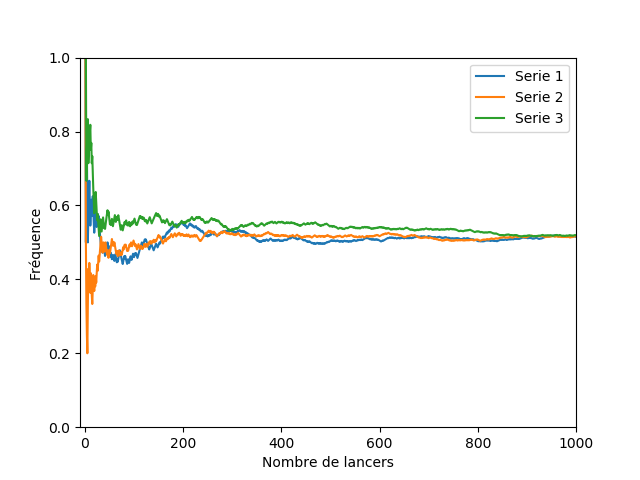
\includegraphics[width=8cm]{frequence_lancer.png}
\end{center}
Le théorème de la loi des grands nombres permet de justifier ce résultat en interprétant la probabilité comme une fréquence de réalisation.\\
La modélisation de cette expérience aléatoire est :
\begin{enumerate}
\item  \impo{n\up{ième} lancer} :  pour tout $n\in\N^*$,  la variable aléatoire $X_n$, représente le résultat du n\up{ième} lancer. Elle  suit une loi Bernouilli de paramètre $p$ sachant que l'issue 0 représente le pile au n\up{ième} lancer et l'issue 1 le face au n\up{ième} lancer. Elles sont supposées indépendantes.  On a $E(X_n) = (1 - p).0 + p.1  = p.$ 
\item \impo{fréquence} : pour tout $n\in\N^*$,  la variable aléatoire $S_n$, représente la moyenne des résultats obtenus au cours des n premiers lancers, soit :
$$ S_n =\frac{X_1+X_2+\dots+X_n}{n}$$ 
\end{enumerate}
L'issue, $\omega$, correspondant à une succession de faces existe. Dans ce cas, $X_n(\omega)=1$ pour tout $n\in \N^*$. Donc $1$ est une valeur possible de la variable aléatoire $S_n$. 
Cependant, le théorème de la loi faible des grands nombres affirme que la probabilité que $S_n$ s'écarte de l'espérance $E(X_n)$ tend vers 0 quand $n$ tend vers l'infini. \\
La loi faible des grands nombres démontre que la probabilité d'un événement peut être définie comme la fréquence théorique vers laquelle tend la
fréquence observée de cet événement lorsque le nombre n de répétitions tend vers l'infini.

\begin{Theoreme}[Loi faible des grands nombres]
Soit $(X_n)_{n\in\N^*}$ une suite de variables aléatoires discrètes définies sur un espace probabilisé $(\Omega,\mathcal{A} ,P)$. On
suppose toutes les variables indépendantes et de même loi, admettant une espérance $m$ et un écart
type $\sigma$. Posons $S_n =\frac{X_1+X_2+\dots+X_n}{n}.$\\
Alors 
$$ \forall \epsilon>0: \quad P\left(\left| S_n - m \right|\geq \epsilon \right )\xrightarrow[n\to+\infty]{}0.$$
\end{Theoreme}
\begin{Demonstration}
D'après l'inégalité de Bienaymé-Tchebychev et par indépendance des variables aléatoires,
$$ \forall \epsilon>0: \quad P\left(\left| S_n - m \right|\geq \epsilon\right)\leq \frac{V(S_n)}{\epsilon^2}=\frac{\frac{V(X_1+X_2+\dots+X_n)}{n^2}}{\epsilon^2}=\frac{\sigma^2}{n\epsilon^2} \xrightarrow[n\to+\infty]{}0.$$
\end{Demonstration}
\begin{Remarque}
Le TP Python \url{https://github.com/VincentTariel/cours/blob/master/probabilite/simulation_variable_aleatoire_avtivite_python.pdf} permet de vous familiariser avec ce théorème sur des applications.
\end{Remarque}
Rapidement, on tombe sur le problème suivant : combien de
lancers de pièces (ou combien de personnes doit on
interroger), pour que le résultat que l'on avance soit correct
avec grosse probabilité... En d'autres termes, on aimerait connaitre "la vitesse" de
convergence. C'est l'objet d'un autre cours sur le théorème centrale limite.
\end{document}
